\chapter{Modeling}
The objective of this thesis is the grouping of expenses with the methods of \ac{NLP}. Grouping, or clustering, is the practise of sorting data points into groups in such a way that the similarity inside a group (intra-cluster similarity) is high while the similarity between clusters (inter-cluster similarity) is low. The defintion of similarity as well as different clustering algorithms are presented and contrasted in the following sections.

\section{Similarity and distance measures}
A distance measure is a quantification of how near objects in space are. Distance measures can be defined for spaces of arbitrary numbers of dimensions. 

		\subparagraph{Euclidean Distance} \label{euclidean}
		The most intuitive and popular distance measure is the euclidean distance. This measure is applicable for vector spaces $F^{n}$ with $n \in \mathbb{N}_0 $. For low-dimensional applications, this distance works well and shows great results. Euclidean distance can be calculated in a highly efficient manner, even for n dimensions. This suggests, that euclidean distance is particularly suitable for high-dimensional data. Unfortunately, euclidean distance falls victim to the curse of dimensionality. In \cite{beyerNearestNeighbor} it is proven that with increasing dimensions, the distance between data points approaches an uniform value for all datapoints. This effect could be demonstrated for spaces with as little as ten dimensions. Therefore, it can be said that euclidean distance is not suitable for high-dimensional data. With vectors in \ac{NLP} ranging from 100 to 800 dimensions, this distance measure is not suitable.
		
		\subparagraph{Dot Product}
		
		
		\subparagraph{Cosine Distance}
		
\section{Clustering Algorithms}
		
		\subsection{K-Means with Euclidean Distance}
		\subsection{DBSCAN}
		
		 \begin{figure}[ht]
			\centering
			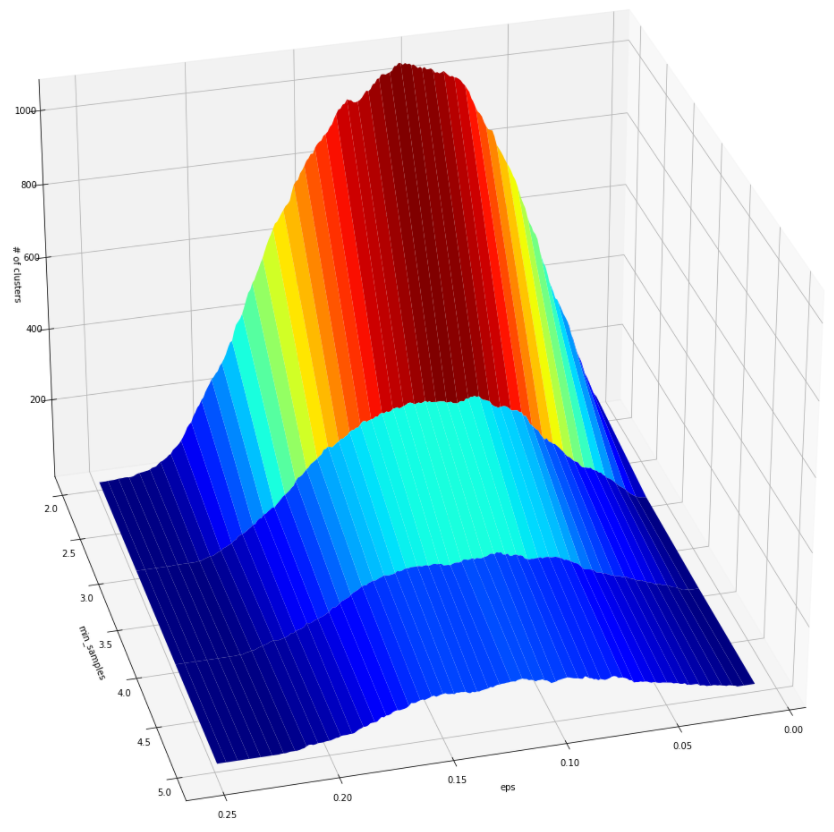
\includegraphics[height=8cm]{Bilder/dbscan_plot.png}
			\caption{DBSCAN hyperparameters and resulting number of clusters}
			\label{fig:dbscan-plot}
		\end{figure}
		
		\subsection{Machine Learning}
		Already Alan Turing understood that for laymen a learning machine can be perceived as a paradox.  How can a machine learn, if a human has to define its behavior beforehand? There are three major subfields in the discipline of artificial intelligence that fundamentally explain how a computer can learn how to behave despite predefined behavior.
		
		\subsection{Supervised Learning}
		A supervised learning algorithm learns its decision with the help of a data set (input) that also contains the correct decision (output) as information. It is trained with only a part of the entire data set, so that the model can be tested in a later step with the help of unknown data. This way, a statement can be made about the accuracy of the model.
		
		\subsection{Unupervised Learning}
		Unsupervised learning is complementary to supervised learning. All algorithms that fall into the category of unsupervised learning are trained with data that does not contain the correct output (label) as information. Here, the categorization is not constrained by the given data, but decided on by the algorithm.
		
		\subsection{Reinforcement Learning}
		The third way in which an algorithm can make better decisions as it gains experience is called reinforcement learning. Reinforcement learning is about letting algorithms solve very complex tasks. The special feature is that there is no defined solution path, but the algorithm is rewarded for goal-oriented behavior and punished for wrong decisions. The definition of goal-oriented behavior has to be put into place by the engineers setting up the training of the model. Real-world tasks are extremely complex, so not all possible solution paths can be calculated and compared to find the optimal path. Parking a car is a routine task for a human after a few hours of driving, but a computer sees only an infinite set of possibilities for turning angles. This problem can be solved by reinforcement learning. The algorithm is rewarded for each parking attempt where the car ends up seeing in the parking space. For the remaining attempts, the algorithm is penalized. Over many thousands of attempts, the reinforcement learning model is trained in this way.
		
		The three major ways of learning even with previously defined behavior can now be implemented by specific models. For example, there are several ways to create and train a model using Unsupervised Learning.
		